\section{Object Detection with YOLO}
YOLO (\textbf{Y}ou \textbf{O}nly \textbf{L}ook \textbf{O}nce) is a family of single-stage objectors detectors, that got popular for it's detection speed, high accuracy and learning capabilities. The rule of thumb was that one-stage detector traded off localization and recognition for a better inference speed, however YOLOv2 manage to change this traditional expectation by outperforming the then state-of-the-art two stage detector, Faster R-CNN \cite{yolov2_paper}. With YOLOv3 this difference became even more clear \cite{yolov3_vs}.

It is important to note, that there are multiple versions such as
YOLOv3 \cite{yolov3_paper}, YOLOv4 \cite{yolov4_paper} and YOLOv7 \cite{yolov7_paper}, but each version may also have multiple implementations e.g. for YOLOv3 there is the Darknet implementation \cite{darknet_git} and also the implementation by Ultralytics \cite{yolov3_ultralytics_git}. One established implementation, that proved good results with a huge community and many features, is the Ultralytics YOLOv5 implementation \cite{yolov5_git}.


\subsection{YOLO architecture}

In this subsection the general architecture and features of more current YOLO detectors will be presented and some significant differences between versions will be highlighted. \\
Current YOLO networks have three main components: the backbone, the neck and the head. From a high-level point of view, the backbone extracts features from an input image, then the neck takes the features from the backbone at different stages and tries to aggregate or distinguish those features to finally pass them to the head. The head has a simple role to generate the predictions i.e. the bounding boxes with the respective confidence score. \\
In YOLOv2 the backbone was just a simple network of 19 convolutional layers and 5 max pooling layers, simply named Darknet-19 \cite{yolov2_paper}. In the next  version, the backbone had very straightforward improvement idea: increase the depth of the network. The new feature extractor is called Darknet-53 and as the name suggests, it had 53 convolutional layers \cite{yolov3_paper}. In YOLOv4, the Darknet-53 is modified to use CSPNet, which lead to the creation of CSPDarknet53. In order to reduce parameters and layers without impacting performance, YOLOv5 replaced the first three layers from CSPDarknet53 with a Focus layer \cite{yolov5_focus}. \\

\begin{figure}
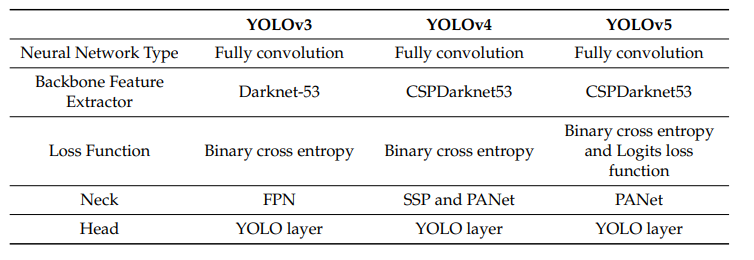
\includegraphics[width=\textwidth]{images/yolo_images/yolo_compare}
\caption{An overview of the structure of YOLOv3-5 networks.}
\end{figure}

The neck component was first used in YOLOv3 with a simple feature pyramid network (FPN), which was then replaced by a PANet SPP network \cite{panet_paper, spp_paper}, but in YOLOv5 the neck is a PANet FPN network. \\
The head is the single component that remained unchanged. The head is just a small fully convolutional network, known as YOLO head, that predicts the bounding boxes. The YOLO head has some parameters, called anchors, that are used to give the head a rough idea of the general shape of the bounding boxes. Those parameters can be optimized before training.  More details about differences between YOLOv3-5 versions are in \cite{yolo_compare}.\\

TODOs:
-YOLOv5 network size
-poza YOLOv5 network

TODO talk also about EfficientDet maybe

Minor TODOs:\\
-cite or hyperlink dev tools \\
\\
YOLOv5 is a version that not only changed the architecture: YOLOv5 is developed in PyTorch (previous ones used Darknet), online augmentations are supported, the simple console output was replaced with more advanced logging tools (e.g. Tensorboard, Weights \& Biases or ClearML), automatic anchor optimization multiple model formats can be used (e.g. ONXX, PyTorch, Tensorflow Lite). In a nutshell, it improved greatly the development experience and speed. \\
This thesis uses YOLOv5, because it outperforms YOLOv1-4 \cite{yolovx_paper} and comes with nice features for development as mentioned above. Of course there are some versions, that were not even mentioned such as YOLOR \cite{yolor_paper} and \cite{yolovx_paper}, but YOLOv5 at the time of writing was the most mature and overall established project. \\


\begin{figure}[!h]
  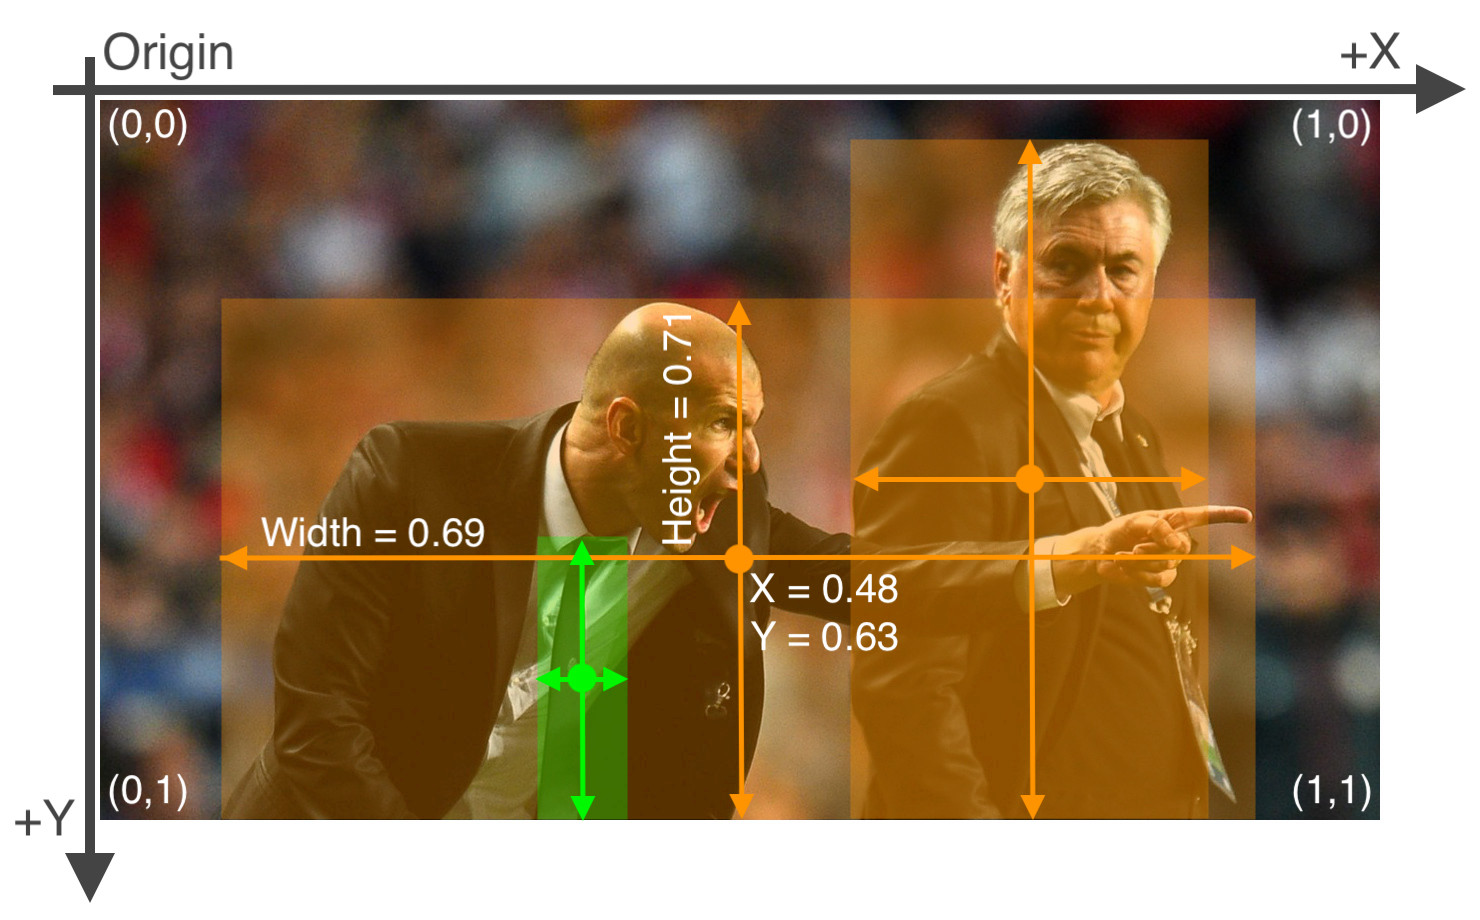
\includegraphics[width=\textwidth]{images/yolo_images/yolo_labels_zidane}
  \centering
  \caption{Example of YOLO bounding box \cite{yolov5_train_custom}}
\end{figure}

\subsection{Labels}
YOLO detectors generally use a distinctive format that consists of 5 mandatory and 1 optional values: \textit{x, y, w, h, class, conf (optional)}. The first 2 values \textit{(x, y)} are the coordinates of the center of the bounding box normalized with respect to the width and height of the image. The next values \textit{w,h} are the width and height of the bounding box, also normalized with respect to the width and height of the image. The next value \textit{class} is the class id. Finally, the value \textit{conf} is used only for detected bounding box to store the confidence of the detection. If \textit{conf} is not given, then it can be assumed that the bounding box is a ground truth and not a detection. Each version might have a slight variation of this notation format, but conceptually they are all the same. \\
This format make the labels invariant to changes of image ratio and resolution.

\subsection{Metrics \& Benchmarks}
In this section some key concepts regarding the evaluation of detections will be defined in order to avoid any sort of confusion and then the evaluation metrics will be presented. \\
The first key concept is the Intersection over Union (IoU), which expresses, how good the overlap between a detection and ground truth bounding box is. The IoU divides the overlap area by the union area, as visualized in figure \ref{fig:iou}.

\begin{figure}[!hb]

  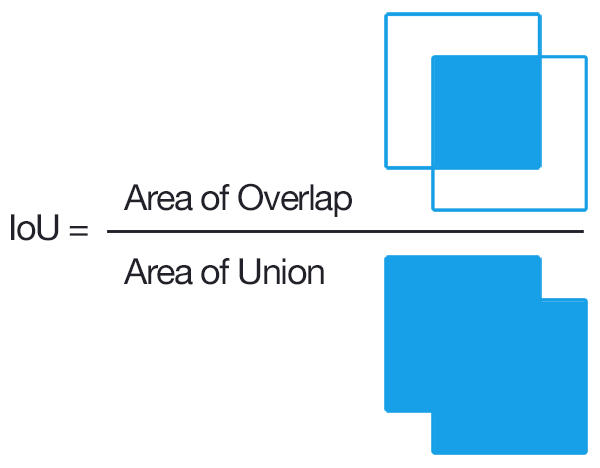
\includegraphics[width=0.75\textwidth]{images/iou}
  \centering
  \caption{IoU formula \cite{map_tutorial}}
  \label{fig:iou}
\end{figure}

The second key concept is the classification of detections in true positive, false positive, false negative. This can be done by taking each detection and seeing, if it has a high IoU with a ground truth bounding box. For a high IoU (i.e. $IoU \geq 0.5$) , then the detection is considered a true positive, else it's a false postive. If a ground truth bounding box is not overlapped by any detections, then the respective missing detection is classified as false negative.\\
Now the metrics precision and recall can be defined:
\begin{equation}
p(c,i) = \frac{TP}{TP + FP}
\end{equation}
\begin{equation}
r(c,i) = \frac{TP}{TP + FN}
\end{equation}
where:
\begin{itemize}
\item[-]{TP = true positives count}
\item[-]{FP = false positives count}
\item[-]{FN = false negatives count}
\item[-]{c = threshold for the confidence of the detections}
\item[-]{i = threshold for the IoU values}
\end{itemize}

The $c$ parameter can be adjusted to improve the recall or precision, which makes sometimes the comparison between two models unclear. Setting the same $conf$ in order to compare two models seems a good approach, but this naive approach might not work, if the models have very different distributions of the confidence values e.g. one model is overconfident and the other one is underconfident. \\
In YOLOv5, this problem was solved by calculating for each model the precision and recall based on the confidence that maximizes the F1-score  \cite{yolov5_conf}:

\begin{equation}
F1(c,i) = 2 * \frac{ p(c,i) * r(c,i)}{p(c,i) + r(c,i)}
\end{equation}

This way a manipulation of the threshold of the confidence values can be avoided and therefor a fairer comparison between models is guaranteed. One caveat of this approach is the assumption that precision and recall have the same importance e.g. an autonomous car needs a higher recall at the detection of red lights. Another caveat of this approach is that it reduces the performance of the model to a single threshold value, but the mean average precison ($mAP$) can be used to express a more general performance. \\
As the name suggests, the $mAP$ is based on the average precision ($AP$), which is calculated indivudually for each class. The AP for a class $C$ and a IoU threshold $i$ can be calculated as follows:

\begin{equation}
AP_C(i) = \sum_{c}{(r(c_{n},i) - r({c_{n-1},i}))p(c_n, i)}
\end{equation}
where $c_n$ are ordered values of confidence thresholds. Finally the mAP is expressed as:
\begin{equation}
mAP(i) = \sum_{C \in classes}{AP_C(i)}
\end{equation}
The IoU threshold can be obviously be lowered to increase the mAP, but usually models are compared for at a threshold of 0.5 and the notation $mAP@0.5$ is preffered. \\
A final metric is the average mAP, usually denoted as $mAP@[0.5:0.95]$. This is just the average $mAP$ for $IoU$ thresholds ranged in 0.5 to 0.95 with a 0.05 step size. \\
For real time object detection application the inference speed is also relevant. The usual benchmark is the number of processed frames per second (FPS) with a resolution of 640x640 or 1280x1280. However, in this project a few frames per seconds is more than enough, since a 3D printers can take at least multiple seconds to print a single layer. Therefore the FPS benchmark will not be discussed or analyzed very much.
